%%%%%%%%%%%%%%%%%%%%%%%%%%%%%%%%%%%%%%%%%%%%%%%%%%%%%%%%%
%%%  整数对象
%%%%%%%%%%%%%%%%%%%%%%%%%%%%%%%%%%%%%%%%%%%%%%%%%%%%%%%%%
\chapter{Python 整数对象}
在 Python2 和 Python3 两个大版本中,对整数的内部实现发生了比较大的变化,在 Python2 中,整数分为两
类,PyIntObject 和 PyLongObject,但是在 Python3 中,整数对象完全由 PyLongObject 来实现,抛弃了
PyIntObject。Python3 中的整数对象定义在文件 longobject.h 中,由 PyLongObject 来实现,先来看一下它的具体定义。

\begin{lstlisting}[language=C, numbers=left, numbersep=1em, numberstyle=\footnotesize , breaklines=true]
// Include/longobject.h
typedef struct _longobject PyLongObject; 

// Include/longintrepr.h
struct _longobject {
    PyObject_VAR_HEAD
    digit ob_digit[1];
};
\end{lstlisting}

实现非常的简单,PyObject\_VAR\_HEAD 表示 PyLongObject 是一个变长对象,大小不是固定的,这个很容易推理,
我们知道,Python 的整数大小几乎是没有上限的,Python 又是使用 C 来实现,C 中没有任何一个基本类型可以放下
一个无限大小的整数,所以,Python 整数必然是使用一个变长对象来实现。把上面的 \_longobject 定义中的宏进行展开。

\begin{lstlisting}[language=C, numbers=left, numbersep=1em, numberstyle=\footnotesize , breaklines=true]
struct _longobject {
	struct {
    		PyObject ob_base;
    		Py_ssize_t ob_size;
	} PyVarObject;
    digit ob_digit[1];
};
\end{lstlisting}

其中的 digit 就是 uint32\_t 的别名。

\begin{figure}[htbp]
\centering
  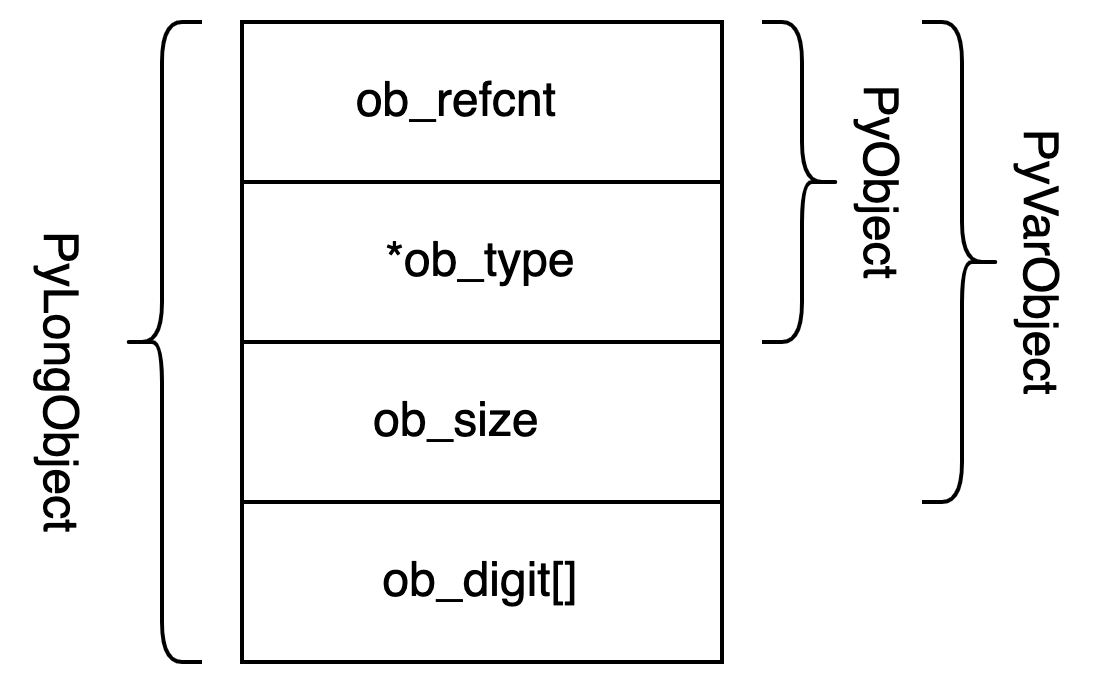
\includegraphics[width=0.5\textwidth]{pictures/ch5_01.png}
  \caption{PyLongObject 的结构 \label{fig:scatter}}
\end{figure}

在这个结构中,很容易看出可变的部分就是指 ob\_digit 数组。根据 \_longobject 结构体的注释,我们可以很轻松地
了解在 Python 中一个整数是怎么样表示的,下面我使用伪代码进行表示。

\begin{algorithm}
\caption{Python 中整数的表示}
$val = 0$\;
\If{$ob\_size == 0$}{
	\Return{0}\;
}
\For{$i \leftarrow 0$ \KwTo $\left|ob\_size \right| - 1$}{
	$val = val + ob\_digit\left[ i \right] \times 2^{SHIFT \times i}$\;
}
\If{$ob\_size > 0$}{
	\Return{$val$}\;
}
\Else{
	\Return{$-val$}
}
\end{algorithm}

算法还是简单易懂的,ob\_size 表示的是整数的符号和 ob\_digit 数组的大小。如果 ob\_size 等于 0 的话那么整数
值就是 0,如果 ob\_size 不等于 0,那么整数的符号就是 ob\_size 的符号,整数的绝对值就等于通过 ob\_digit 计算出来
的值。ob\_digit 的计算规则稍微复杂一点,所以我们通过例子来进行讲解。首先要说明一下伪代码中 SHIFT 这个值的含义。

在 Python 中,有一个叫做 PYLONG\_BITS\_IN\_DIGIT 的宏,表示 Python 整数对象中的 ob\_digit 数组的每个元素使用
的字节长度,如果 PYLONG\_BITS\_IN\_DIGIT 等于 30,那么 ob\_digit 数组就是一个 uint32\_t 数组,每个数组元素的
长度为 4 字节(32 位),如果 PYLONG\_BITS\_IN\_DIGIT 等于 15,那么 ob\_digit 数组就是一个 unsigned short 数组,每个数组
元素的长度为 2 字节(16 位)。PYLONG\_BITS\_IN\_DIGIT 的值表示 PyLongObject 使用 ob\_digit 数组成员的位数。
如果是uint32\_t 数组,那么对数组中的每个元素,只使用其中的 30 位,如果是 unsigned short 数组,对于数组中的每个成员,
只使用其中的 15 位。空出来的几位的作用是什么,下面会讲到。有两种定义的原因是考虑到不同机器的 int 长度不一样,
在 32 位机器喜爱,int 的长度是 2 字节,在 64 位机器下,int 的长度是 4 字节,需要针对不同的硬件做不同的调整。下面
的介绍中,如果没有特殊说明,默认 PYLONG\_BITS\_IN\_DIGIT 的值为 30。

现在可以告诉你了,上面伪代码中的 SHIFT 就是 PYLONG\_BITS\_IN\_DIGIT。现在有如下几个 PyLongObject 对象,来
计算一下它们表示的整数值。

\begin{figure}[htbp]
\centering
  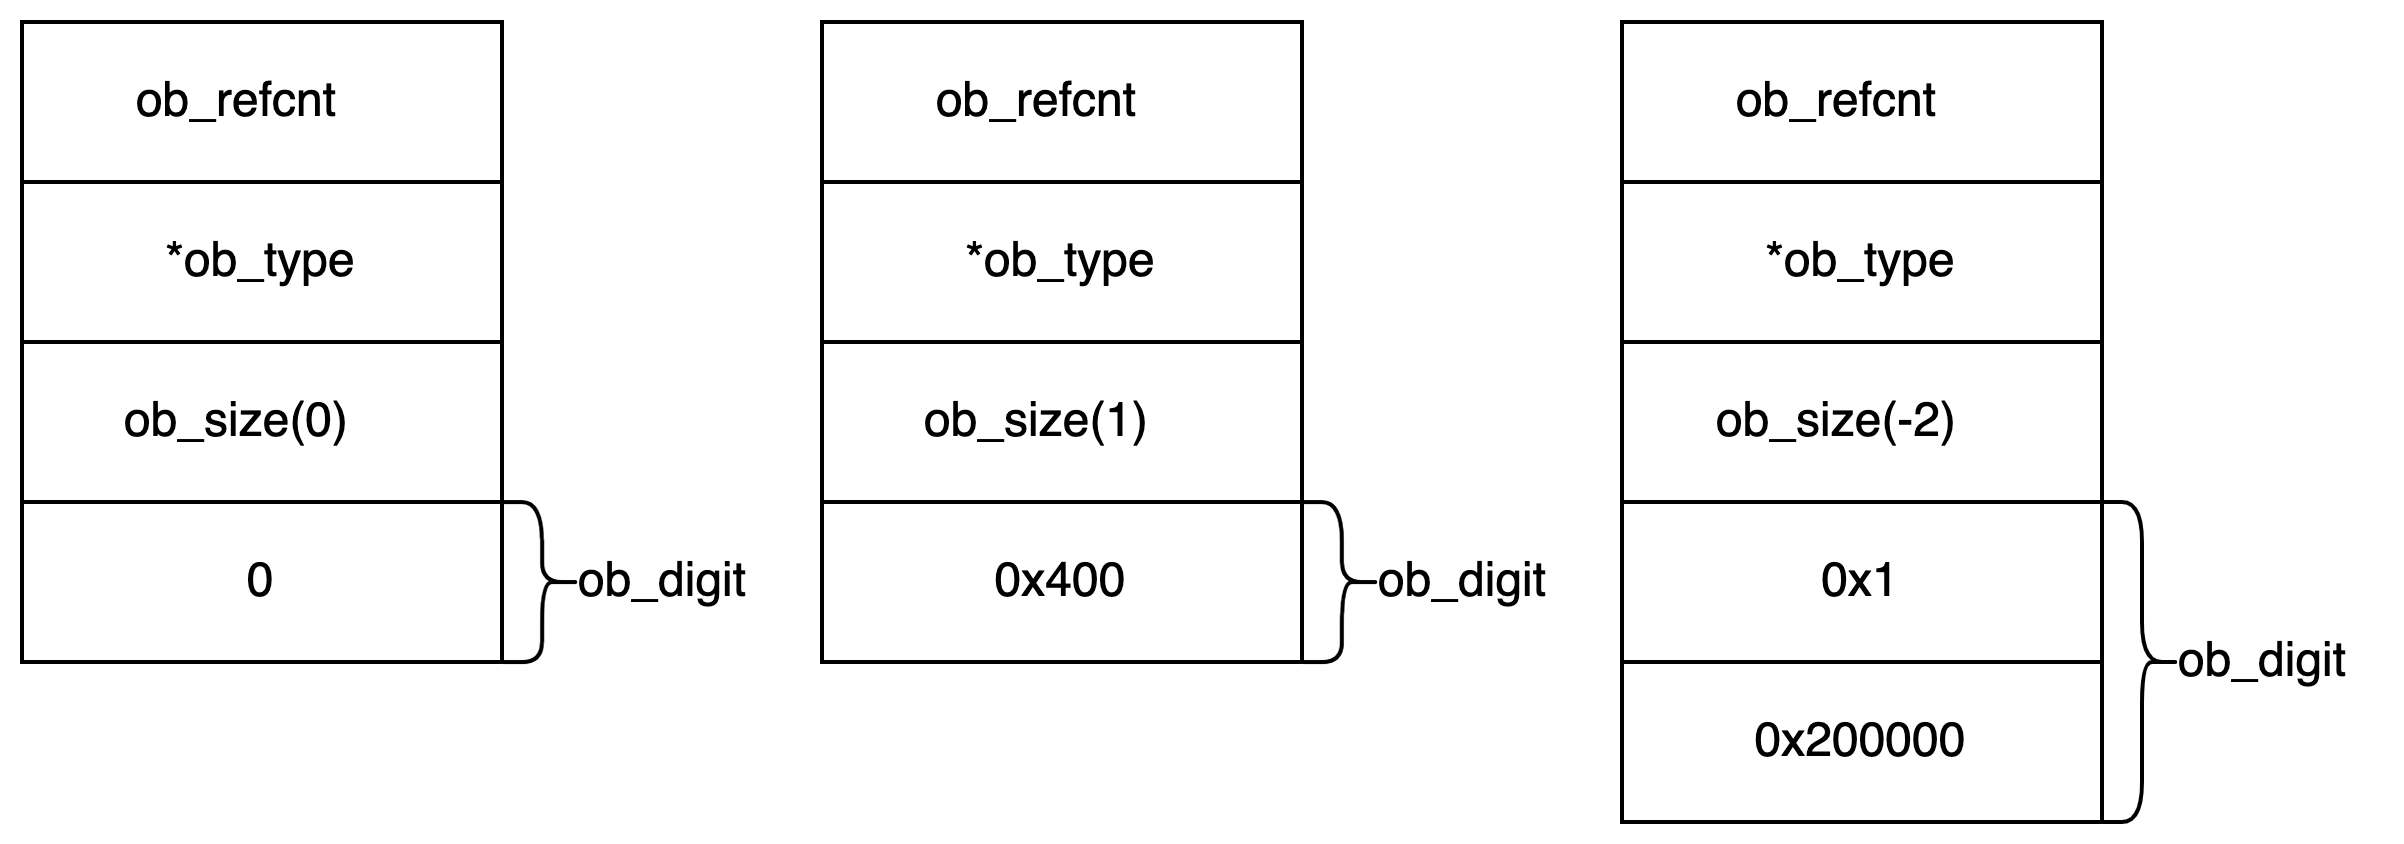
\includegraphics[width=0.8\textwidth]{pictures/ch5_02.png}
  \caption{3 个 PyLongObject 例子 \label{fig:scatter}}
\end{figure}

第一个 PyLongObject 中 ob\_size 等于 0,所以它表示的整数值就是 0 了。第二个 PyLongObject 中 ob\_size 等于 1,所以表示
的是一个正整数,ob\_size 等于 1 也说明 ob\_digit 数组的长度为 1,所以这个整数的值就是 0x400,也就是10进制整数 1024。
第三个 PyLongObject 中 ob\_size 等于 -2,说明这是一个负整数,并且 ob\_digit 数组的长度等于 2,根据 ob\_digit 数组和上面
伪代码给出的公式,算出整数的绝对值等于 $0x1 + 0x200000 \times 2^{30} = 2251799813685249$,所以第三个 PyLongObject 表示的整数
值就是 -2251799813685249。

下面是编写的2个函数,分别用来将一个整数转化为 ob\_size 和 ob\_digit,或者将 ob\_size 和 ob\_digit 转化为整数。
可以利用这组函数来验证上面对 PyLongObject 中整数值计算方法的描述。

\begin{lstlisting}[language=Python, numbers=left, numbersep=1em, numberstyle=\footnotesize , breaklines=true]
def int_2_digits(n:int):
    mod = 2**30
    flag = 1 if n >= 0 else -1
    ob_size = 0
    digits = []
    n = abs(n)
    
    while n > 0:
        digits.append(n % mod)
        n = n // mod
        ob_size += 1

    ob_size = flag * ob_size
    return ob_size, digits

def digits_2_int(ob_size:int, digits:list):
    SHIFT = 30
    n = 0
    if ob_size == 0:
        return n

    for i in range(abs(ob_size)):
        n += digits[i] * (2 ** (SHIFT * i))

    return n if ob_size > 0 else -n

def print_digits(n:int):
    ob_size, digits = int_2_digits(n)
    new_n = digits_2_int(ob_size, digits)
    digits = [hex(i) for i in digits]
    print("n:{} ob_size:{} digits:{} new_n:{}".format(n, ob_size, digits, new_n))
    assert n == new_n, "n:{} ob_size:{} digits:{} new_n:{}".format(n, ob_size, digits, new_n)

# 测试例子
print_digits(2**10)
print_digits(-(2**51+1))
\end{lstlisting}


\section{Python 中创建 PyLongObject 对象的几种方式}

Python 中,有多种方式可以创建一个 PyLongObject 对象,这些方式都定义在 longobject.h 文件中。

\begin{lstlisting}[language=C, numbers=left, numbersep=1em, numberstyle=\footnotesize , breaklines=true]
// Include/longobject.h
PyAPI_FUNC(PyObject *) PyLong_FromLong(long);
PyAPI_FUNC(PyObject *) PyLong_FromUnsignedLong(unsigned long);
PyAPI_FUNC(PyObject *) PyLong_FromSize_t(size_t);
PyAPI_FUNC(PyObject *) PyLong_FromSsize_t(Py_ssize_t);
PyAPI_FUNC(PyObject *) PyLong_FromDouble(double);
PyAPI_FUNC(PyObject *) PyLong_FromLongLong(long long);
PyAPI_FUNC(PyObject *) PyLong_FromUnsignedLongLong(unsigned long long);
// 省略掉其他一些
\end{lstlisting}

下面分析一下其中的几个例子。

\begin{lstlisting}[language=C, numbers=left, numbersep=1em, numberstyle=\footnotesize , breaklines=true]
// Objects/longobject.c
PyObject *
PyLong_FromLong(long ival)
{
    PyLongObject *v;
    // 保存 ival 的绝对值
    unsigned long abs_ival;
    unsigned long t;  /* unsigned so >> doesn't propagate sign bit */
    int ndigits = 0;
    int sign;
	// 如果是小整数那么直接返回小整数池中的对象
    if (IS_SMALL_INT(ival)) {
        return get_small_int((sdigit)ival);
    }
	// 如果 ival 是一个负数的话,是不可以通过取它的负数 -ival
	// 来获取绝对值,因为如果 ival = LONG_MIN 的话,-ival会溢出
    if (ival < 0) {
        abs_ival = 0U-(unsigned long)ival;
        sign = -1;
    }
    else {
        abs_ival = (unsigned long)ival;
        // 这里是一个亮点,记得上面提到过 ob_size 等于 0
        // 的话表示 PyLongObject 保存的整数值为 0 吗?
        sign = ival == 0 ? 0 : 1;
    }
    // 如果 ival 的绝对值使用一个 ob_digit 数组元素可以
    // 存下的话,那么进入快速通道
    if (!(abs_ival >> PyLong_SHIFT)) {
        v = _PyLong_New(1);
        if (v) {
            Py_SET_SIZE(v, sign);
            v->ob_digit[0] = Py_SAFE_DOWNCAST(
                abs_ival, unsigned long, digit);
        }
        return (PyObject*)v;
    }

// 如果 PyLong_SHIFT == 15 并且 abs_ival 可以使用两个 ob_digit 数组元素存下的话
// 则进行处理,类似上面的快速通道
#if PyLong_SHIFT==15
    /* 2 digits */
    if (!(abs_ival >> 2*PyLong_SHIFT)) {
        v = _PyLong_New(2);
        if (v) {
            Py_SET_SIZE(v, 2 * sign);
            v->ob_digit[0] = Py_SAFE_DOWNCAST(
                abs_ival & PyLong_MASK, unsigned long, digit);
            v->ob_digit[1] = Py_SAFE_DOWNCAST(
                  abs_ival >> PyLong_SHIFT, unsigned long, digit);
        }
        return (PyObject*)v;
    }
#endif

    // 这一步计算需要使用多少个元素的 ob_digit 数组可以放在这个整数
    t = abs_ival;
    while (t) {
        ++ndigits;
        t >>= PyLong_SHIFT;
    }
    v = _PyLong_New(ndigits);
    if (v != NULL) {
        digit *p = v->ob_digit;
        Py_SET_SIZE(v, ndigits * sign);
        t = abs_ival;
        // 对 PyLongObject 的 ob_digit 数组进行赋值
        while (t) {
            *p++ = Py_SAFE_DOWNCAST(
                t & PyLong_MASK, unsigned long, digit);
            t >>= PyLong_SHIFT;
        }
    }
    return (PyObject *)v;
}
\end{lstlisting}

上面的代码可以看出 PyLong\_FromLong 如何将一个 long 类型的整数转化为一个 PyLongObject 对象。
在 PyLong\_FromLong 函数里面,可以看到是使用 \_PyLong\_New 来创建一个 PyLongObject 对象,并且
给这个函数传递一个表示 ob\_digit 数组大小的参数。下面看看在它的内部究竟是做了什么操作才构造出
了一个 PyLongObject 对象。

\begin{lstlisting}[language=C, numbers=left, numbersep=1em, numberstyle=\footnotesize , breaklines=true]
// Objects/longobject.c
PyLongObject *
_PyLong_New(Py_ssize_t size)
{
    PyLongObject *result;
    // 如果申请的 ob_digit 数组的大小超过了 MAX_LONG_DIGITS,则抛出异常 
    if (size > (Py_ssize_t)MAX_LONG_DIGITS) {
        PyErr_SetString(PyExc_OverflowError,
                        "too many digits in integer");
        return NULL;
    }
    // 申请 PyLongObject 需要的内存大小
    result = PyObject_Malloc(offsetof(PyLongObject, ob_digit) +
                             size*sizeof(digit));
    if (!result) {
        PyErr_NoMemory();
        return NULL;
    }
    // 初始化 PyLongObject 对象
    _PyObject_InitVar((PyVarObject*)result, &PyLong_Type, size);
    return result;
}
\end{lstlisting}

\_PyLong\_New 函数的内容一目了然,主要包含两个步骤,申请内存和初始化 PyLongObject 对象。
在复制代码中时候,删除了关于申请内存处的一个注释,注释主要是说在之前的版本中,计算需要
申请的内存大小的方式是计算 sizeof(PyVarObject) + sizeof(digit)*size,但是在这个版本中使用的方式
是 offsetof(PyLongObject, ob\_digit) + sizeof(digit)*size,做这个改变的原因是在某些机器或者操作系统
中,使用 sizeof 计算可能会因为内存对齐导致计算的大小比实际的大小要大一些。为了验证这个说法,
下面写了一段简单的代码。

\begin{lstlisting}[language=C, numbers=left, numbersep=1em, numberstyle=\footnotesize , breaklines=true]
#include <stdio.h>
#include <stddef.h>
#include <stdint.h>

typedef ssize_t         Py_ssize_t;
typedef uint32_t digit;

typedef struct _object {
  Py_ssize_t ob_refcnt;
  void *ob_type; // 使用 void* 代替 PyTypeObject*
} PyObject;

typedef struct {
  PyObject ob_base;
  Py_ssize_t ob_size; /* Number of items in variable part */
} PyVarObject;

#define PyObject_VAR_HEAD      PyVarObject ob_base;

struct _longobject {
  PyObject_VAR_HEAD
  digit ob_digit[1];
};

typedef struct _longobject PyLongObject;

int main() {
  int n1 = sizeof(PyVarObject);
  int n2 = offsetof(PyLongObject, ob_digit);
  printf("n1=%d, n2=%d\n", n1, n2); /
  return 0;
}
\end{lstlisting}

但是在我的机器上输入结果是 $n1=24, n2=24$,两种计算方式并没有差异。
在在线编译器测试平台\\
 https://godbolt.org/ 上实验了多个编译器,也没有差异。
如果感兴趣的话,可以自己编译这一段代码试试看。

接下来继续看另一个创建 PyLongObject 对象的函数 PyLong\_FromDouble。这个函数中会用到 C
标准库中的 frexp 和 ldexp 函数,所以先对它进行一下介绍。frexp 函数的声明如下。

\begin{lstlisting}[language=C, numbers=left, numbersep=1em, numberstyle=\footnotesize , breaklines=true]
double frexp(double value, int *exp);

double ldexp(double x, int n);
\end{lstlisting}

frexp 函数会把浮点数参数 value 分解成为一个归一化的小数(就是frexp 函数的返回值,记做 ret,值的范围为 0 
和 $[\frac{1}{2}, 1)$)和 2 的整数幂(保存在 exp 中)。这两个数和 value 的关系是 $value = x \times 2^{exp} $。
ldexp 函数会计算 $ret = x \times 2^{n}$,其中 ret 是 ldexp 函数的返回值。了解了这个知识,继续看
PyLong\_FromDouble 函数吧。

\begin{lstlisting}[language=C, numbers=left, numbersep=1em, numberstyle=\footnotesize , breaklines=true]
PyObject *
PyLong_FromDouble(double dval)
{
    // 如果dval 的值在 long 的范围之内,调用 PyLong_FromLong 函数进行构造
    const double int_max = (unsigned long)LONG_MAX + 1;
    if (-int_max < dval && dval < int_max) {
        return PyLong_FromLong((long)dval);
    }

    PyLongObject *v;
    double frac;
    int i, ndig, expo, neg;
    neg = 0; // 表示是否是一个负数
    // 如果 dval 是 inf,抛出异常,返回 NULL
    if (Py_IS_INFINITY(dval)) {
        PyErr_SetString(PyExc_OverflowError,
                        "cannot convert float infinity to integer");
        return NULL;
    }
    // 如果 dval 是 nan,抛出异常,返回 NULL
    if (Py_IS_NAN(dval)) {
        PyErr_SetString(PyExc_ValueError,
                        "cannot convert float NaN to integer");
        return NULL;
    }
    if (dval < 0.0) {
        neg = 1;
        dval = -dval;
    }
    frac = frexp(dval, &expo); /* dval = frac*2**expo; 0.0 <= frac < 1.0 */
    assert(expo > 0);
    ndig = (expo-1) / PyLong_SHIFT + 1; /* Number of 'digits' in result */
    v = _PyLong_New(ndig);
    if (v == NULL)
        return NULL;
    frac = ldexp(frac, (expo-1) % PyLong_SHIFT + 1);
    for (i = ndig; --i >= 0; ) {
        digit bits = (digit)frac;
        v->ob_digit[i] = bits;
        frac = frac - (double)bits;
        frac = ldexp(frac, PyLong_SHIFT);
    }
    if (neg) {
        Py_SET_SIZE(v, -(Py_SIZE(v)));
    }
    return (PyObject *)v;
}
\end{lstlisting}

这个函数中比较难理解的部分是计算 ob\_digit 数组的值,将这一部分代码单独抽离出来看一下。

\begin{lstlisting}[language=C, numbers=left, numbersep=1em, numberstyle=\footnotesize , breaklines=true]
#include <stdio.h>
#include <math.h>
#include <inttypes.h>

#define PyLong_SHIFT 30
typedef uint32_t digit;

int main() {
  double dval = 6.917529027641082e+17; // 0.6 * 2**60
  double frac;
  int i, ndig, expo;

  frac = frexp(dval, &expo);
  // 计算出要用多少个 ob_digit 数组元素才可以保存下 double 的整数部分
  ndig = (expo-1) / PyLong_SHIFT + 1;
  frac = ldexp(frac, (expo-1) % PyLong_SHIFT + 1);
  for (i = ndig; --i >= 0;) { // 对 ob_digit 数组从高位到低位赋值
    digit bits = (digit)frac; // bits 就是 frac 的整数部分
    printf("%u ", bits);
    frac = frac - (double)bits; // frac 等于原来的 frac 的小数部分
    frac = ldexp(frac, PyLong_SHIFT); // frac = frac * 2**30
  }
  printf("\n");

  return 0;
}
\end{lstlisting}

编译执行上面这个 C 程序的输出如下。
\begin{lstlisting}[language=bash, numbers=left, numbersep=1em, numberstyle=\footnotesize , breaklines=true]
644245094 429496704
\end{lstlisting}

ob\_digit[1] = 644245094, ob\_digit[0] = 429496704。

PyLong\_FromDouble 函数之所以要如此大费周张的使用 frexp, ldexp 函数来进行计算,原因其实很简单:C 语言中没有任何一种整数
类型可以存储的下 double 的所有可能值整数部分,这样子是不是一下子就理解了。


\subsection{小整数池}

前面在快速通道的地方提到了小整数池,那么这一节就继续探究一下小整数池的内容。

\begin{lstlisting}[language=C, numbers=left, numbersep=1em, numberstyle=\footnotesize , breaklines=true]
#define _PY_NSMALLPOSINTS           257
#define _PY_NSMALLNEGINTS           5

#define NSMALLNEGINTS           _PY_NSMALLNEGINTS
#define NSMALLPOSINTS           _PY_NSMALLPOSINTS

#define IS_SMALL_INT(ival) (-NSMALLNEGINTS <= (ival) && (ival) < NSMALLPOSINTS)

PyObject *
PyLong_FromLong(long ival)
{
	// ... ...
    if (IS_SMALL_INT(ival)) {
        return get_small_int((sdigit)ival);
    }
    // ... ...
}
\end{lstlisting}

IS\_SMALL\_INT 宏用来判断一个整数是不是小整数,小整数的范围是 $[-5,\ 257)$。如果一个整数
在这个范围内的话,那么 PyLong\_FromLong 函数就会调用 get\_small\_int 函数来返回一个 PyLongObject。

\begin{lstlisting}[language=C, numbers=left, numbersep=1em, numberstyle=\footnotesize , breaklines=true]
// Objects/longobject.c
static PyObject *
get_small_int(sdigit ival)
{
    assert(IS_SMALL_INT(ival));
    PyObject *v = __PyLong_GetSmallInt_internal(ival);
    Py_INCREF(v);
    return v;
}

static inline PyObject* __PyLong_GetSmallInt_internal(int value)
{
    PyInterpreterState *interp = _PyInterpreterState_GET();
    assert(-_PY_NSMALLNEGINTS <= value && value < _PY_NSMALLPOSINTS);
    size_t index = _PY_NSMALLNEGINTS + value;
    // 直接从 interp->small_ints 数组中获取缓存的 PyLongObject 对象
    PyObject *obj = (PyObject*)interp->small_ints[index];
    assert(obj != NULL);
    return obj;
}

\end{lstlisting}

interp->small\_ints 的初始化是在 \_PyLong\_Init 中实现的,可以看到其中使用一个 for 循环,生成了 5 + 257 个 PyLongObject
对象保存在 small\_ints 数组中。

\begin{lstlisting}[language=C, numbers=left, numbersep=1em, numberstyle=\footnotesize , breaklines=true]
int
_PyLong_Init(PyInterpreterState *interp)
{
    for (Py_ssize_t i=0; i < NSMALLNEGINTS + NSMALLPOSINTS; i++) {
        sdigit ival = (sdigit)i - NSMALLNEGINTS;
        int size = (ival < 0) ? -1 : ((ival == 0) ? 0 : 1);

        PyLongObject *v = _PyLong_New(1);
        if (!v) {
            return -1;
        }

        Py_SET_SIZE(v, size);
        v->ob_digit[0] = (digit)abs(ival);

        interp->small_ints[i] = v;
    }
    return 0;
}
\end{lstlisting}




\section{参考资料}

\begin{itemize}
\item \href{https://flaggo.github.io/python3-source-code-analysis/objects/long-object/}{Python 整数对象}
\item \href{https://godbolt.org/}{Compiler Explorer}
\end{itemize}
